\documentclass[11pt,a4paper]{article}
\usepackage[T1]{fontenc}
\usepackage[utf8]{inputenc}
\usepackage{lmodern}
\usepackage{babel}
\babelprovide[import,main]{french}
\usepackage[margin=2.15cm,top=2.2cm,bottom=2.1cm,headheight=15pt]{geometry}
\usepackage{microtype,amsmath,amssymb,mathtools,graphicx}
\usepackage[table]{xcolor}
\usepackage{booktabs,tabularx,array,enumitem,caption,fancyhdr,lastpage}
\usepackage[most]{tcolorbox}
\usepackage{tikz}
\usepackage{titlesec}
\usepackage{hyperref}
\usepackage{xurl}
\definecolor{navy}{HTML}{173044}
\definecolor{teal}{HTML}{087E8B}
\definecolor{gold}{HTML}{AD8444}
\definecolor{pale}{HTML}{EEF5F6}
\definecolor{graytext}{HTML}{52636F}
\hypersetup{colorlinks=true,linkcolor=teal,urlcolor=teal,citecolor=teal,
 pdftitle={Complétion de données pour Laplace~: synthèse de trois études},
 pdfauthor={Halhoul Mhamed},pdfsubject={Projet scientifique de Master - synthèse scientifique},
 pdfkeywords={problèmes inverses, Laplace, apprentissage statistique, régularisation, covariance}}
\urlstyle{same}
\setlength{\parindent}{0pt}
\setlength{\parskip}{6pt}
\linespread{1.06}
\setlist{nosep,leftmargin=1.4em,topsep=3pt,itemsep=3pt}
\setlength{\tabcolsep}{5pt}
\renewcommand{\arraystretch}{1.22}
\newcolumntype{Y}{>{\raggedright\arraybackslash}X}
\titleformat{\section}{\Large\sffamily\bfseries\color{navy}}{\thesection}{.6em}{}
\titleformat{\subsection}{\normalsize\sffamily\bfseries\color{teal}}{\thesubsection}{.6em}{}
\titlespacing*{\section}{0pt}{0pt}{12pt}
\titlespacing*{\subsection}{0pt}{10pt}{4pt}
\captionsetup{font=small,labelfont=bf,labelsep=period,hypcap=false}
\pagestyle{fancy}\fancyhf{}
\fancyhead[L]{\footnotesize\sffamily\color{graytext}LAPLACE \enspace / \enspace SYNTHÈSE DES TROIS ÉTUDES}
\fancyhead[R]{\footnotesize\sffamily\color{graytext}Halhoul Mhamed}
\fancyfoot[L]{\scriptsize\color{graytext}Projet scientifique de Master \enspace | \enspace 11 octobre 2026}
\fancyfoot[R]{\scriptsize\color{graytext}\thepage\,/\,\pageref*{LastPage}}
\renewcommand{\headrulewidth}{.35pt}
\renewcommand{\footrulewidth}{0pt}
\newtcolorbox{keybox}[1][]{colback=pale,colframe=teal,boxrule=.45pt,arc=1mm,
 left=10pt,right=10pt,top=7pt,bottom=7pt,fonttitle=\sffamily\bfseries,coltitle=navy,
 colbacktitle=pale,enhanced,title=#1}
\newcommand{\src}[1]{\textcolor{graytext}{\footnotesize #1}}
\newcommand{\RR}{\mathcal R}
\newcommand{\E}{\mathbb E}
\newcommand{\repo}{https://github.com/halhoulmhamed-droid/inverse-laplace-learning}
\newcommand{\shaone}{0ea95cd7e390c8a478469b36a043a5f99e4fcd10}
\newcommand{\shatwo}{57ab54ebc994029be3c24a8a34da56371547f4ac}
\newcommand{\shathree}{867144db98eba3c0f5fe7cece4261918a46f1c31}
\newcommand{\gitlink}[3]{\href{\repo/blob/#1/#2}{#3}}
\DeclareRobustCommand{\eref}[1]{\hyperlink{ref#1}{[#1]}}
\begin{document}

% COUVERTURE
\begin{titlepage}
\hypersetup{pageanchor=false}
\thispagestyle{empty}
\begin{minipage}[c]{.68\textwidth}

\includegraphics[width=7.3cm]{assets/logos/uae.png}
\end{minipage}\hfill
\begin{minipage}[c]{.23\textwidth}\raggedleft

\includegraphics[height=2.35cm]{assets/logos/fpl.png}
\end{minipage}
\vspace{.7cm}
\begin{center}
{\large\sffamily\bfseries\color{navy}Université Abdelmalek Essaâdi}\par
{\normalsize Faculté Polydisciplinaire de Larache}\par
\vspace{1.35cm}
{\small\sffamily\bfseries\color{teal}PROJET SCIENTIFIQUE DE MASTER}\par
\vspace{.65cm}
{\fontsize{26}{31}\selectfont\sffamily\bfseries\color{navy}
Complétion de données\par pour l'équation de Laplace}\par
\vspace{.55cm}
{\Large\sffamily\color{graytext}Apprentissage, covariances\par et régularisation}\par
\vspace{.65cm}
{\large\sffamily\bfseries\color{teal}Synthèse cohérente des trois études}\par
\vspace{.6cm}
{\color{gold}\rule{3cm}{1.2pt}}\par
\vspace{.6cm}
{\Large\bfseries Halhoul Mhamed}\par
\vspace{.35cm}
Master\par
\textit{Modélisation mathématique et applications et apprentissages}\par
M2 en cours\par
\end{center}
\vfill
\begin{center}
\textbf{Professeur encadrant~: Pr. Chakir Tajani}\par
\vspace{.4cm}
11 octobre 2026\par
\vspace{.4cm}
{\small\color{graytext}Synthèse des résultats archivés, destinée à la discussion scientifique.}\par
{\small\href{\repo}{github.com/halhoulmhamed-droid/inverse-laplace-learning}}
\end{center}
\end{titlepage}
\hypersetup{pageanchor=true}
\setcounter{page}{1}

\section{Résumé et fil conducteur}
\begin{keybox}[Résultat d'ensemble]
Les trois études montrent que l'intérêt d'un estimateur appris dépend de ce qui est appris,
de l'espace de reconstruction et du protocole d'évaluation. Un bénéfice ciblé des covariances
complètes est établi dans l'étude 2. Ni le plafonnement des gains de l'étude 1 ni le mélange
de covariance de l'étude 3 ne démontrent le bénéfice utile attendu dans leur contraste principal.
Ces conclusions sont compatibles.
\end{keybox}

Le problème commun est de reconstruire une trace supérieure inconnue à partir de mesures
bruitées prises sur le bord inférieur d'un domaine harmonique. Les hautes fréquences sont
fortement atténuées par le modèle direct. L'apprentissage fournit une information statistique
sur les signaux~; la régularisation limite l'instabilité, au prix d'un biais possible.

\begin{tabularx}{\textwidth}{@{}p{.11\textwidth}YYY@{}}
\toprule
\textbf{Étude} & \textbf{Question principale} & \textbf{Constat rapporté} & \textbf{Verdict limité}\\
\midrule
1 & Le plafond améliore-t-il le filtre appris signé~? & Ratios du quantile 95\,\% proches de 1. & Gain utile de 10\,\% non établi.\\
\addlinespace
2 & Les blocs de covariance complets aident-ils à espace fixé~? & Risque F/D~: 0,3192 à 0,3218. & Gain ciblé établi selon le protocole.\\
\addlinespace
3 & Mélanger la covariance vers une cible $H^1$ aide-t-il~? & Rapport des risques moyens S/M0~: 0,9720. & Gain utile de 3\,\% non établi~; protection satisfaite.\\
\bottomrule
\end{tabularx}
\src{Sources~: \eref{E1}, p.~8--10~; \eref{E2}, p.~5--7~; \eref{E3}, p.~6--8. Les pages citées sont les numéros imprimés des rapports.}

\subsection*{Trois questions successives, sans classement artificiel}
\textbf{Étude 1~: stabilité.} Diminuer l'amplification du bruit par une borne sur les gains
ne suffit pas à garantir une amélioration du risque total.

\textbf{Étude 2~: représentation.} À entrées et sorties identiques, exploiter les blocs de
covariance complets peut améliorer la reconstruction. La prédiction hors du sous-espace
retenu constitue un effet supplémentaire à isoler.

\textbf{Étude 3~: estimation.} Une covariance empirique peut elle-même être régularisée.
Le bénéfice observé dépend alors de la cible, de la taille d'apprentissage et du réglage.

\subsection*{Portée de cette synthèse}
Ce document rassemble les trois rapports fournis et leurs liens scientifiques. Il ne constitue
ni une nouvelle campagne ni une reproduction indépendante des pertes brutes. Les graphiques
ci-après sont des transcriptions de tableaux publiés dans les rapports. Les comparaisons
confirmatoires restent séparées des constats secondaires. Le code, la chronologie des gels
et les audits annoncés ne sont pas réaudités intégralement dans cette synthèse.

\newpage
\section{Le problème inverse et le rôle de l'apprentissage}
Sur $\Omega_H=(0,1)\times(0,H)$, avec $H=1/4$ au nominal, le potentiel satisfait
\[
\Delta u=0,\qquad u(x,H)=q(x),\qquad
\partial_nu=0\quad\text{sur les bords inférieur et latéraux}.
\]
La trace supérieure $q$ est inconnue. Les flux nuls sont une hypothèse du modèle~; ils ne
sont pas des mesures exactes obtenues gratuitement. Les capteurs mesurent des moyennes
de $u(\cdot,0)$ sur 64 intervalles, avant sélection éventuelle d'un masque. \eref{E1}

Dans la base orthonormée $\phi_0=1$, $\phi_k(x)=\sqrt2\cos(k\pi x)$, le transfert inférieur vaut
\[
q=\sum_{k\geq0}c_k\phi_k,\qquad
T_Hq=\sum_{k\geq0}t_kc_k\phi_k,\qquad
t_0=1,\quad t_k=\operatorname{sech}(k\pi H).
\]
Pour une somme finie, la solution est
\[
u(x,y)=c_0+\sum_{k\geq1}c_k\phi_k(x)
\frac{\cosh(k\pi y)}{\cosh(k\pi H)}.
\]
Comme $t_k\to0$, $T_H$ est compact et injectif sur $L^2$, mais son inverse sur son image
n'est pas borné. La petite perturbation $t_k\phi_k$ dans les observations correspond à une
perturbation $\phi_k$ de norme 1 dans la trace inconnue. C'est l'instabilité du problème inverse.
Ce prolongement du transfert sur $L^2$ n'affirme pas une régularité énergétique jusqu'au bord
supérieur pour toute trace $L^2$.

\subsection*{Modèle continu, acquisition et calcul numérique}
Les trois études distinguent le générateur analytique à 128 coefficients et l'opérateur inverse
nominal en différences finies à 64 coefficients, sur 64\,$\times$\,16 intervalles. La troncature,
la discrétisation, le masque et une erreur de hauteur peuvent donc affecter la reconstruction.
L'injectivité du transfert continu n'implique pas l'identifiabilité de toute trace à partir d'un
nombre fini de capteurs. \eref{E1}\eref{E2}\eref{E3}

\subsection*{Ce qui est appris}
Les méthodes considérées sont des \textbf{estimateurs affines appris}, de la forme
\[
\widehat c=\mu_c+R(y-\mu_y).
\]
L'apprentissage estime des moyennes, des covariances, des covariances croisées ou des gains
spectraux~; la validation choisit les paramètres de régularisation. Il s'agit d'apprentissage
statistique, sans réseau neuronal profond dans ces trois études.

\begin{keybox}[Information statistique et information physique]
Une distribution d'apprentissage peut rendre certaines directions prévisibles en moyenne.
Elle ne transforme pas une direction non observable en information déterministe présente
dans chaque mesure. Une reconstruction statistiquement plausible doit donc rester distinguée
d'une identification garantie pour tout signal.
\end{keybox}

\newpage
\section{Des protocoles reliés, mais non interchangeables}
Les études partagent le problème physique et un générateur nominal à coefficients cosinus
indépendants. Elles changent cependant la question testée, l'information utilisée pour régler
les méthodes et la définition de la perte. \eref{E1}\eref{E2}\eref{E3}

{\small
\begin{tabularx}{\textwidth}{@{}p{.21\textwidth}YYY@{}}
\toprule
 & \textbf{Étude 1} & \textbf{Étude 2} & \textbf{Étude 3}\\
\midrule
Comparaison & Signé plafonné / signé & F / D, rang 12 commun & S / M0, covariance du signal\\
\addlinespace
Apprentissage & 1\,000 objets~; 3 jeux & 64, 256, 1\,024~; 5 jeux & 32, 64, 256~; 5 jeux\\
\addlinespace
Taille principale & 1\,000 & 256 & 64\\
\addlinespace
Validation & 200 objets~; deux observations~; pas de vérité pour le réglage & 256 objets~; deux bruits~; vérité synthétique autorisée & 256 objets~; deux bruits~; vérité synthétique autorisée\\
\addlinespace
Test & 200 objets par régime~; 10 bruits & 400 objets~; 4 bruits & 400 nouveaux objets~; 4 bruits\\
\addlinespace
Bruit & Niveau relatif au RMS d'apprentissage & Écart-type absolu~; $\sigma=0,01$ au principal & Écart-type absolu~; $\sigma=0,01$ au principal\\
\addlinespace
Perte principale & Erreur relative $L^2$~; quantile 95\,\% & Erreur quadratique $L^2$ moyenne & Erreur quadratique $L^2$ moyenne\\
\addlinespace
Rééchantillonnage & 2\,000 bootstraps par objets & 4\,000 bootstraps par objets & 4\,000 bootstraps par objets\\
\bottomrule
\end{tabularx}}

\subsection*{L'unité statistique est l'objet physique}
Les répétitions de bruit et les méthodes appliquées au même objet sont dépendantes. Les
études 2 et 3 moyennent les quatre pertes de bruit avant d'évaluer le risque sur 400 objets.
Le bootstrap conserve l'appariement. Les cinq entraînements partagent les objets de test :
ils ne créent pas 2\,000 objets indépendants.

\subsection*{Des seuils préfixés, avec une portée conditionnelle}
L'étude 1 utilise des bornes à 98,75\,\% et une correction pour quatre inégalités par
entraînement~; elle ne revendique pas de couverture simultanée sur les trois entraînements.
Les études 2 et 3 utilisent des bornes à 99,5\,\% et dix inégalités corrigées par Bonferroni.
Ces bornes bootstrap restent approximatives et conditionnelles aux ajustements observés.

\begin{keybox}[Règle de lecture]
Les ratios de chaque étude comparent ses propres méthodes sur ses propres données.
On ne peut ni additionner les gains ni comparer directement 68\,\% et 2,8\,\% pour classer
les trois études. Une baisse de risque quadratique n'est pas la même chose qu'une baisse
de norme d'erreur, de médiane ou de quantile.
\end{keybox}

\newpage
\section{Étude 1~: borner les gains ne suffit pas}
\subsection*{Hypothèse et mécanisme}
Dans une représentation singulière, le filtre appris signé utilise des gains $g_j$.
Le plafonnement remplace ces gains par des valeurs de module au plus $C$.
Pour $R=V_r\operatorname{diag}(g_j)U_r^\top$, on a
\[
\|R\|_2=\max_j|g_j|.
\]
Réduire cette norme limite l'amplification du bruit. Mais, dans le cas centré simplifié
$y=Ac+\varepsilon$, l'erreur s'écrit
\[
\widehat c-c=(RA-I)c+R\varepsilon.
\]
La modification de $R$ agit simultanément sur le biais et sur le terme de bruit. Dans le modèle
effectif s'ajoutent les erreurs de discrétisation, les modes omis et les différences de centrage.
Une meilleure borne de stabilité n'impose donc pas une meilleure erreur de reconstruction.
\eref{E1}, p.~6--7.

\subsection*{Contraste et résultat principal}
Le protocole exige une borne supérieure du ratio des quantiles 95\,\% \textbf{strictement
inférieure à 0,90}, avec une borne du ratio de médiane nominale associée inférieure à 1,05.
Les deux situations principales sont P1, avec 32 capteurs contigus nominaux, et P2, avec
capteurs complets et hauteur augmentée de 5\,\%, au niveau de bruit principal de 1\,\%.

\begin{center}\small
\begin{tabular}{@{}lrrr@{}}
\toprule
 & \textbf{Jeu 0} & \textbf{Jeu 1} & \textbf{Jeu 2}\\
\midrule
P1~: ratio observé $q_{95}$ & 0,97096 & 0,98498 & 0,98987\\
P1~: borne supérieure & 0,99908 & 1,00117 & 1,00308\\
P2~: ratio observé et borne & 1,00000 & 1,00000 & 1,00000\\
\bottomrule
\end{tabular}\end{center}
\src{Transcription de \eref{E1}, p.~9. Ratios~: filtre signé plafonné / filtre signé.}

\begin{keybox}[Conclusion de l'étude 1]
Aucune des six évaluations principales ne démontre le gain utile attendu du plafond.
Les protections de médiane sont respectées, mais le critère portant sur le quantile ne l'est pas.
Il s'agit d'un résultat comparatif non concluant pour ce bénéfice, et non d'un échec numérique
ni d'une preuve d'absence de tout effet.
\end{keybox}

\subsection*{Pourquoi poursuivre avec les covariances~?}
Les comparaisons secondaires suggèrent que la forme de la pénalité et la famille d'estimateurs
peuvent compter davantage que le seul plafond. Toutefois, comparer un filtre diagonal à un
estimateur complet peut changer à la fois les dépendances exploitées et l'espace de sortie.
L'étude 2 a donc pour objet de séparer ces effets, avec un nouveau protocole explicite.

\src{Provenance~: \gitlink{\shaone}{results/analysis/primary.json}{résultats principaux},
\gitlink{\shaone}{results/analysis/bootstrap.npz}{bootstrap},
\gitlink{\shaone}{docs/protocol.md}{protocole} et
\gitlink{\shaone}{results/full/configuration.json}{configuration} au commit \texttt{0ea95cd7e390}.}

\newpage
\section{Étude 2~: un gain ciblé des blocs complets}
La comparaison principale impose les mêmes espaces d'entrée et de sortie de rang $r=12$.
Avec $z=U_r^\top(y-\mu_y)$, $b=V_r^\top(c-\mu_c)$ et
$t=\operatorname{tr}(C_{zz})/r$, les opérateurs sont
\begin{align*}
R_F&=V_rC_{bz}(C_{zz}+\lambda tI)^{-1}U_r^\top,\\
R_D&=V_r\operatorname{diag}\!\left(
\frac{\operatorname{diag}C_{bz}}{\operatorname{diag}C_{zz}+\lambda t}\right)U_r^\top.
\end{align*}
F exploite les deux blocs complets~; D les diagonalise. Cette comparaison ne sépare pas
l'apport individuel de chaque bloc. \eref{E2}, p.~3.

\subsection*{Le résultat confirmatoire}
Avec 32 capteurs contigus, $N=256$ et $\sigma=0,01$, les cinq ratios de risque F/D vont
de \textbf{0,3192 à 0,3218}. Leurs bornes supérieures vont de 0,3301 à 0,3350, sous le seuil
0,95. Les cinq protections du quantile passent également le seuil 1,05. Le bénéfice est donc
établi selon la règle annoncée, conditionnellement aux cinq entraînements observés.
La baisse d'environ \textbf{68\,\% concerne le risque quadratique}, pas chaque erreur individuelle.
\eref{E2}, p.~5--6.

\begin{center}
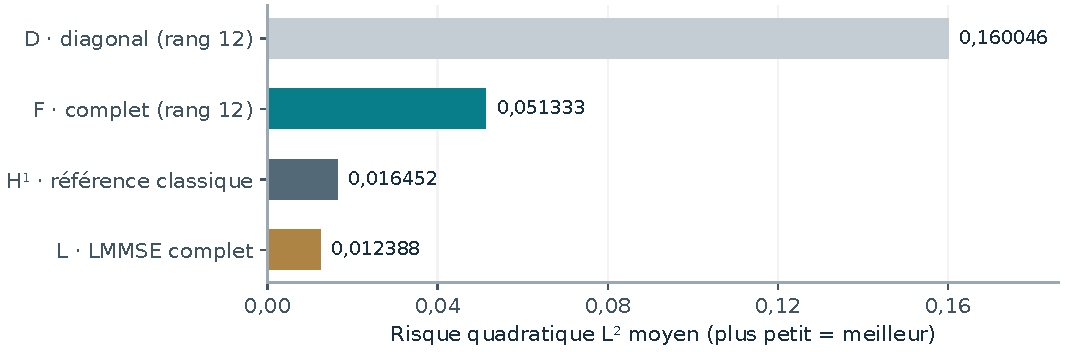
\includegraphics[width=.97\textwidth]{figures/etude2_risques.pdf}
\captionof{figure}{Risques moyens du scénario principal de l'étude 2. Les valeurs sont transcrites
du tableau de \eref{E2}, p.~7. Seul F/D est le contraste confirmatoire~; H$^1$ et L situent
des comparaisons secondaires. Il ne s'agit pas d'une nouvelle simulation.}
\end{center}
\src{Simulation d'origine :
\gitlink{\shatwo}{studies/study2/results/analysis/summary.csv}{données},
\gitlink{\shatwo}{studies/study2/src/figures.py}{script},
\gitlink{\shatwo}{studies/study2/results/final/configuration.json}{configuration}.
Version~: \href{\repo/tree/\shatwo}{\texttt{57ab54ebc994}}.}

\subsection*{Un succès local ne signifie pas une supériorité générale}
F reste moins bon que la référence $H^1$ dans ce scénario~: 0,051333 contre 0,016452.
Le LMMSE complet L atteint 0,012388~; son avantage sur $H^1$ est \emph{secondaire et descriptif}.
Il présente aussi des dégradations dans d'autres scénarios, notamment avec observations
complètes ou rugosité accrue.

Les coefficients cosinus physiques sont indépendants dans le générateur. Les covariances
hors diagonale en base singulière proviennent notamment de la représentation et du masque.
Le résultat ne démontre pas la découverte de corrélations physiques nouvelles.

\newpage
\section{Étude 3~: régulariser la covariance apprise}
L'étude 3 teste un mélange de covariance du signal dans la base cosinus :
\[
C_\gamma=(1-\gamma)C_{\rm emp}+\gamma C_{H^1},\quad
C_{H^1}=sQ^{-1},\quad Q=\operatorname{diag}(1+(\pi k)^2),\quad
s=\frac{\operatorname{tr}C_{\rm emp}}{\operatorname{tr}Q^{-1}}.
\]
L'opérateur et les observations sont divisés par 8~; la variance du bruit devient
$\nu=\sigma^2/64$. Avec $\beta=\alpha\nu>0$, l'opérateur et le centre sont
\[
R_{\gamma,\alpha}=C_\gamma A^\top(AC_\gamma A^\top+\beta I)^{-1},
\qquad \widehat c=\mu+R_{\gamma,\alpha}(y-A\mu).
\]
S règle $\gamma$ et $\alpha$~; M0 fixe $\gamma=0$ et règle $\alpha$.
La matrice à inverser est définie positive grâce à $\beta I$, même lorsque
$C_{\rm emp}$ est singulière. La cible a la même trace que la covariance empirique,
mais sa décroissance en $k^{-2}$ diffère de celle du générateur nominal, proche de $k^{-5}$.
\eref{E3}, p.~3--5.

\begin{center}
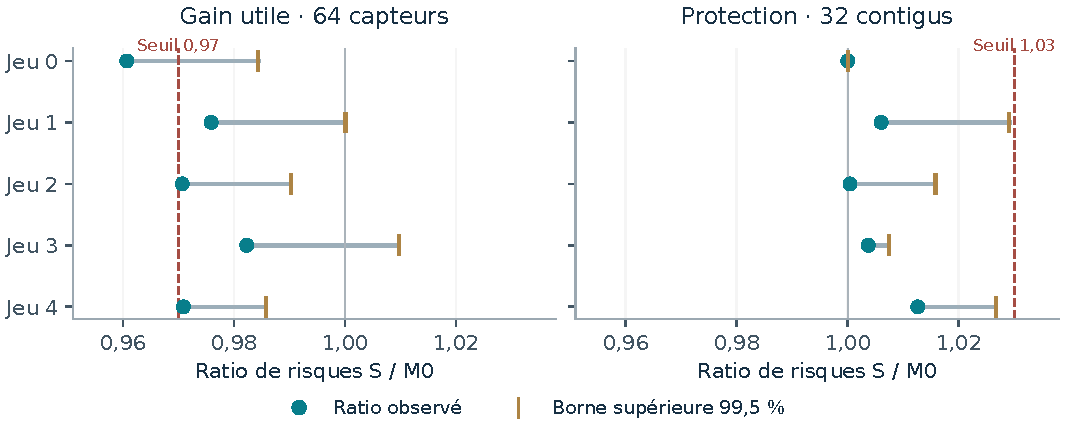
\includegraphics[width=\textwidth]{figures/etude3_criteres.pdf}
\captionof{figure}{Décision principale de l'étude 3, à $N=64$, $\sigma=0,01$.
Les segments relient l'estimation à sa borne supérieure~: ce ne sont pas des intervalles
bilatéraux. Valeurs arrondies transcrites de \eref{E3}, p.~6.}
\end{center}
\src{Simulation d'origine :
\gitlink{\shathree}{studies/study3/figures/primary.npz}{données},
\gitlink{\shathree}{studies/study3/src/figures.py}{script},
\gitlink{\shathree}{studies/study3/results/final/configuration.json}{configuration}.
Version~: \href{\repo/tree/\shathree}{\texttt{867144db98eb}}.}

\subsection*{Un bénéfice descriptif, mais pas le gain utile requis}
En complet, le rapport des risques moyens est \textbf{0,9720}, soit une baisse descriptive
de 2,8\,\%. Aucune des cinq bornes supérieures ne passe sous 0,97~: le gain utile de 3\,\%
n'est pas établi. Sur 32 capteurs contigus, toutes les bornes restent sous 1,03~; la protection
est satisfaite, avec un rapport des risques moyens de 1,0045, soit environ 0,45\,\% de dégradation.

À $N=32$, le ratio secondaire 0,9283 suggère un bénéfice plus visible avec moins de données.
Il ne remplace pas le résultat principal après coup. La covariance diagonale en base cosinus
fait mieux que S dans les cinq entraînements nominaux, complets et contigus. Le mélange
se dégrade aussi sous certaines perturbations de rugosité ou de hauteur. \eref{E3}, p.~7--10.

\newpage
\section{Interprétation commune~: ce que les études isolent}
\subsection*{1. Contrôler l'amplification et réduire le risque sont distincts}
L'étude 1 illustre le compromis biais--variance. Une contrainte sur les gains peut améliorer
une borne d'amplification sans réduire assez l'erreur observée. Un résultat favorable sur une
propriété d'opérateur ne remplace pas une évaluation de reconstruction.

\subsection*{2. La covariance dépend de la base et de l'espace de sortie}
Dans l'étude 2, le bénéfice F/D est mesuré dans un sous-espace commun. La sortie complète
de O ou L apporte une possibilité différente~: prédire statistiquement des composantes hors
de ce sous-espace. À même paramètre, les identités de projection distinguent ces mécanismes.
Le complément du sous-espace de rang 12 n'est pas nécessairement le noyau exact du direct.

Dans l'étude 3, \textbf{Diag n'est pas D}. Diag conserve la diagonale de la covariance du signal
en base cosinus~; D diagonalise des blocs en base singulière dans l'étude 2. Leur classement
différent n'est donc pas une contradiction. \eref{E2}, p.~3, 8--10~; \eref{E3}, p.~4.

\subsection*{3. Changer de famille n'est pas seulement ajouter un mélange}
Le LMMSE empirique E de l'étude 3 appartient à la famille appelée L dans l'étude 2~: il utilise
des covariances signal--observation et un centre d'observation empirique. M0 emploie la
covariance du signal, l'opérateur nominal et le centre $A\mu$. En échantillon fini, ces objets
ne coïncident pas en général.

Ainsi, le ratio descriptif S/E de 0,7549 ne mesure pas le seul effet du mélange. La comparaison
S/M0, de 0,9720 en risques moyens complets, est celle destinée à évaluer cet ajout.
À $\gamma=1$, l'équivalence avec une pénalité $H^1$ nécessite le même centre et la conversion
du paramètre. Elle n'implique pas l'égalité avec le $H^1$ historique sélectionné sur une autre
grille. \eref{E3}, p.~4, 8.

\begin{keybox}[Une formulation scientifique défendable]
Dans un benchmark synthétique de complétion de Laplace, l'exploitation de blocs de covariance
complets apporte un gain important face à une restriction diagonale, dans un contraste à
espaces contrôlés. Ce gain ne se généralise pas à tous les comparateurs et scénarios.
Le plafonnement des gains et la contraction vers une cible $H^1$ n'établissent pas les
bénéfices utiles préfixés dans leurs comparaisons principales respectives.
\end{keybox}

\subsection*{Le lien avec le machine learning}
Le travail étudie l'apprentissage de régularisateurs et d'estimateurs à partir de distributions
de signaux. L'intérêt scientifique repose sur l'analyse des mécanismes, la généralisation
limitée et le contrôle des comparaisons, plutôt que sur la profondeur d'une architecture.
Cette perspective s'inscrit dans les cadres spectraux et quadratiques appris déjà étudiés
dans la littérature. \eref{R1}\eref{R2}

\newpage
\section{Limites communes et niveau de preuve}
\begin{tabularx}{\textwidth}{@{}p{.31\textwidth}Y@{}}
\toprule
\textbf{Limite} & \textbf{Conséquence pour l'interprétation}\\
\midrule
Signaux synthétiques & Les tests ne démontrent pas une performance sur des mesures expérimentales réelles.\\
\addlinespace
Distribution et géométrie limitées & Quelques masques, bruits, rugosités et hauteurs sont étudiés~; pas de robustesse générale.\\
\addlinespace
Peu d'entraînements & Trois ou cinq ajustements ne permettent pas une garantie sur tous les futurs apprentissages.\\
\addlinespace
Bootstrap conditionnel & L'incertitude est approximative et dépend des modèles et validations observés.\\
\addlinespace
Réglage non uniforme entre études & La sélection observationnelle de l'étude 1 et la sélection supervisée des études 2--3 ne sont pas directement équivalentes.\\
\addlinespace
Grilles et comparateurs fixés & Les résultats concernent les procédures testées, et non un optimum illimité de chaque famille.\\
\bottomrule
\end{tabularx}

\subsection*{Deux réserves propres aux comparaisons positives}
\textbf{Étude 2.} Une seule troncature $r=12$ est étudiée. D atteint fréquemment une borne
de sa grille de réglage dans les ajustements rapportés. Cela n'annule pas le contraste préfixé,
mais limite l'interprétation comme supériorité sur toute version possible d'un estimateur diagonal.

\textbf{Étude 3.} S explore 140 candidats, contre 20 pour M0 et chacun des autres
comparateurs. La comparaison réglée porte sur des procédures pratiques de budgets différents.
Les diagnostics à $\alpha$ commun isolent une modification de covariance, mais peuvent
désavantager un M0 auquel on n'accorde plus son propre réglage. Ils restent descriptifs.
\eref{E2}, p.~11~; \eref{E3}, p.~5, 8.

\subsection*{Vérification informatique et résultat scientifique}
Les études 2 et 3 annoncent respectivement 11 et 17 tests ciblés réussis. Les trois rapports
décrivent des contrôles indépendants ciblés. Ces éléments documentent la vérification des implémentations~; ils ne
démontrent pas la supériorité d'une méthode. De même, les millions de reconstructions
comptabilisées incluent répétitions, méthodes et diagnostics~: ce ne sont pas des millions
d'objets indépendants. Cette synthèse reprend ces bilans comme \emph{déclarations des rapports},
sans les transformer en une nouvelle certification.

\subsection*{Contribution et antériorité}
Les méthodes affines, les régularisations quadratiques apprises et la contraction de covariance
ont des antériorités. Le dossier apporte une étude comparative structurée sur un problème
inverse contrôlé, avec des hypothèses explicites et des limites conservées. Il ne démontre
pas une nouveauté algorithmique, ni à lui seul l'originalité requise pour une publication de recherche.

\newpage
\section{Conclusion et discussion avec l'encadrant}
Les trois études forment un parcours scientifique cohérent~: elles distinguent successivement
la maîtrise de l'amplification, le rôle de la représentation statistique et la régularisation de
cette représentation. Elles fournissent un résultat positif local et deux bénéfices utiles non
établis. Conserver ces trois issues est nécessaire pour représenter fidèlement le travail.

\begin{keybox}[Conclusion générale]
L'apprentissage statistique peut améliorer une reconstruction de Laplace dans un cadre
précis, mais son intérêt ne découle ni du seul plafonnement des gains ni de l'ajout automatique
d'une contraction de covariance. Il doit être évalué face à des références correctement réglées,
en distinguant information physique, représentation, estimation et incertitude.
\end{keybox}

\subsection*{Ce que le dossier permet de présenter}
\begin{enumerate}
\item Un problème inverse réellement instable, avec transfert analytique et direct numérique distincts.
\item Des estimateurs appris interprétables, reliés aux covariances et à la régularisation classique.
\item Une séparation entre contrastes principaux, comparaisons secondaires et diagnostics de mécanisme.
\item Un résultat ciblé documenté dans le protocole de l'étude 2, accompagné de ses contre-exemples et limites.
\item Une traçabilité vers les données, scripts, configurations et versions scientifiques.
\end{enumerate}

\subsection*{Questions prioritaires à discuter}
\textbf{Référence pertinente.} Quelle question mérite une confirmation nouvelle face à une
méthode simple et forte~: $H^1$, covariance diagonale en base physique, ou modèle nominal sans mélange~?

\textbf{Information disponible.} Dans l'application envisagée, dispose-t-on de traces propres
pour valider les paramètres, ou seulement de mesures~? Le choix d'un protocole futur doit
refléter cette contrainte.

\textbf{Transfert.} Quelle perturbation a un sens physique prioritaire~: autre hauteur,
bruit corrélé, capteurs mal localisés ou changement de distribution~? Une seule extension
motivée serait plus interprétable qu'une multiplication de scénarios après observation des résultats.

\textbf{Confirmation.} Si une hypothèse nouvelle est retenue, prévoir des données inédites,
des budgets de réglage comparables, une unité statistique explicite et un critère de réussite
fixé avant test. Une telle étude dépasse le périmètre de cette synthèse.

\subsection*{Positionnement académique}
Cette synthèse constitue une base de discussion pour approfondir le travail de Master et
préparer une démarche de recherche. Sa valeur tient à la compréhension et à la défense
des choix mathématiques et expérimentaux. Un résultat positif supplémentaire ne doit pas
devenir une condition imposée aux données.

\newpage
\section{Traçabilité et réutilisation des résultats}
Les liens ci-dessous pointent vers des \textbf{versions scientifiques immuables} plutôt que vers
une branche susceptible d'évoluer. Ils proviennent des annotations des rapports fournis.
Les chemins ont été contrôlés dans les arbres Git correspondants lors de la préparation de
la synthèse~; ce contrôle d'existence ne remplace pas l'audit du contenu des archives.

\subsection*{Étude 1}
\href{\repo/tree/\shaone}{\texttt{\shaone}}\par
\gitlink{\shaone}{docs/protocol.md}{Protocole} \enspace | \enspace
\gitlink{\shaone}{docs/theory.md}{Cadre mathématique} \enspace | \enspace
\gitlink{\shaone}{results/analysis/primary.json}{Résultats principaux}\par
\gitlink{\shaone}{results/analysis/summary.csv}{Tableau des résultats} \enspace | \enspace
\gitlink{\shaone}{results/full/configuration.json}{Configuration} \enspace | \enspace
\gitlink{\shaone}{scripts/figures.py}{Script des figures}

\subsection*{Étude 2}
\href{\repo/tree/\shatwo}{\texttt{\shatwo}}\par
\gitlink{\shatwo}{studies/study2/PROTOCOL.md}{Protocole} \enspace | \enspace
\gitlink{\shatwo}{studies/study2/MATHEMATICS.md}{Cadre mathématique} \enspace | \enspace
\gitlink{\shatwo}{studies/study2/FREEZE.json}{Gel déclaré}\par
\gitlink{\shatwo}{studies/study2/figures/primary.npz}{Données principales} \enspace | \enspace
\gitlink{\shatwo}{studies/study2/figures/projection.npz}{Comparaisons des espaces}\par
\gitlink{\shatwo}{studies/study2/results/final/configuration.json}{Configuration} \enspace | \enspace
\gitlink{\shatwo}{studies/study2/src/figures.py}{Script des figures}

\subsection*{Étude 3}
\href{\repo/tree/\shathree}{\texttt{\shathree}}\par
\gitlink{\shathree}{studies/study3/PROTOCOL.md}{Protocole} \enspace | \enspace
\gitlink{\shathree}{studies/study3/MATHEMATICS.md}{Cadre mathématique} \enspace | \enspace
\gitlink{\shathree}{studies/study3/MATHEMATICS_ADDENDUM.md}{Précision mathématique}\par
\gitlink{\shathree}{studies/study3/figures/primary.npz}{Données principales} \enspace | \enspace
\gitlink{\shathree}{studies/study3/figures/robustness.npz}{Perturbations}\par
\gitlink{\shathree}{studies/study3/results/final/configuration.json}{Configuration} \enspace | \enspace
\gitlink{\shathree}{studies/study3/src/figures.py}{Script des figures}

\subsection*{Reproduire cette synthèse}
Le paquet source contient le fichier LaTeX, les deux logos, les deux figures vectorielles,
leurs CSV de transcription et le script de tracé. La compilation du document ne nécessite
pas de relancer les expériences~: deux passages de \texttt{pdflatex} suffisent avec les figures
fournies. Le script de tracé lit uniquement ces CSV~; il ne calcule aucune reconstruction.

Le fichier \texttt{PROVENANCE.json} conserve les empreintes des trois PDF sources et les
références de leurs tableaux. Le manifeste du paquet identifie les octets livrés. Les nombres
arrondis transcrits ne doivent pas être utilisés pour refaire les tests statistiques~: pour cela,
il faut repartir des archives scientifiques originales et de leurs protocoles.

\newpage
\section*{Références et contact}
\addcontentsline{toc}{section}{Références et contact}
\subsection*{Rapports sources}
\hypertarget{refE1}{}\textbf{[E1] Halhoul Mhamed.}
\textit{Complétion de données pour l'équation de Laplace. Filtrage spectral appris~: stabilité
au bruit et à l'erreur de modèle}. 11 octobre 2026, 16 pages PDF.
Sections 1--10~; principaux résultats p.~8--10. Version scientifique
\href{\repo/tree/\shaone}{\texttt{0ea95cd7e390}}.

\hypertarget{refE2}{}\textbf{[E2] Halhoul Mhamed.}
\textit{Complétion de données de Laplace. Apport des covariances apprises et robustesse
aux observations partielles}. Étude 2, 11 octobre 2026, 13 pages PDF.
Principaux résultats p.~5--7~; projections et limites p.~8--12. Version scientifique
\href{\repo/tree/\shatwo}{\texttt{57ab54ebc994}}.

\hypertarget{refE3}{}\textbf{[E3] Halhoul Mhamed.}
\textit{Étude 3~: régularisation des covariances apprises. Pour une reconstruction robuste
de données de Laplace}. 11 octobre 2026, 13 pages PDF.
Principaux résultats p.~6--8~; perturbations et limites p.~9--12. Version scientifique
\href{\repo/tree/\shathree}{\texttt{867144db98eb}}.

\subsection*{Repères bibliographiques}
\hypertarget{refR1}{}\textbf{[R1] M. Burger et S. Kabri.}
\textit{Learned Regularization for Inverse Problems: Insights from a Spectral Model}.
arXiv:2312.09845v2, 2024.
\href{https://arxiv.org/abs/2312.09845}{Notice et résumé des auteurs}.

\hypertarget{refR2}{}\textbf{[R2] G. S. Alberti, E. De Vito, M. Lassas, L. Ratti et M. Santacesaria.}
\textit{Learning the optimal Tikhonov regularizer for inverse problems}. NeurIPS 2021.
\href{https://proceedings.neurips.cc/paper_files/paper/2021/hash/d3e6cd9f66f2c1d3840ade4161cf7406-Abstract.html}{Notice officielle et résumé}.

\src{Ces deux notices ont été consultées pour situer le cadre. Leurs preuves ne sont pas
réauditées ici~; cette liste n'est pas une revue exhaustive ni un audit de nouveauté.
Les rapports sources conservent leurs bibliographies détaillées et leurs déclarations académiques.}

\subsection*{Identité institutionnelle}
Les logos correspondent à l'Université Abdelmalek Essaâdi et à la Faculté Polydisciplinaire
de Larache. Leur provenance officielle est conservée dans le paquet source. Ils indiquent
l'affiliation~; ils ne constituent pas une validation institutionnelle des conclusions.

\vspace{.15cm}
\begin{keybox}[Contact]
\textbf{Halhoul Mhamed}\par
\href{mailto:halhoul.mhamed@etu.uae.ac.ma}{halhoul.mhamed@etu.uae.ac.ma}\par
\href{mailto:halhoulmhamed@gmail.com}{halhoulmhamed@gmail.com}\par
\href{\repo}{github.com/halhoulmhamed-droid/inverse-laplace-learning}
\end{keybox}
\end{document}
